\section{Question 2}
\subsection{Part a}
$ZP(1,0,1,1)=e^0\cdot e^0 = 1$\\
$ZP(1,1,0,0)=e^0\cdot e^0 = 1$\\
$ZP(1,1,0,1)=e^0\cdot e^1 = e$\\
$ZP(1,1,1,0)=e^1\cdot e^1 = e^2$\\
$ZP(1,1,1,1)=e^1\cdot e^0 = e$\\

\subsection{Part b}
First, $x_1$ is added to the BN. It has no parents. When adding $x_2$, observe that $P(x_1, x_2)=\frac{1}{4}$ for all combinations of $(x_1, x_2)$. This equals $P(x_1)\cdot P(x_2)$. Thus, $x_2\independent x_1$.\\
When $x_3$ is added, given both $x_1$ and $x_2$, the probability that $x_3=x_1\oplus x_2$ is $\frac{1}{e}$ times the probability of $x_3=\neg(x_1\oplus x_2)$. Similarly, $x_3$ is dependent on $x_2$ given $x_1$. Thus, we add edges from $x_1$ and $x_2$ to $x_3$.\\
When $x_4$ is added, given $x_3$, the probability that $x_4=x_3$ is $e$ times the probability that $x_4=\neg x_3$ and is independent of $x_1$ and $x_2$. Thus, we add an edge from $x_3$ to $x_4$.\\
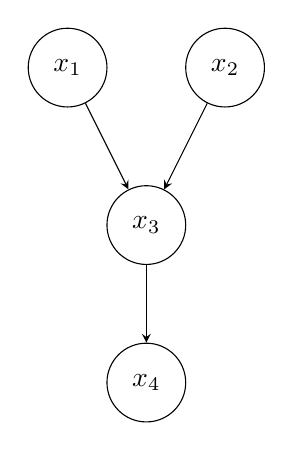
\begin{tikzpicture}[
    node distance=2cm and 2cm, % Adjusts spacing
    every node/.style={draw, circle, minimum size=1cm, text centered},
    >=stealth
]

% Nodes
\node (x1) at (0, 2) {$x_1$};
\node (x2) at (2, 2) {$x_2$};
\node (x3) at (1, 0) {$x_3$};
\node (x4) at (1, -2) {$x_4$};

% Edges
\draw[->] (x1) -- (x3);
\draw[->] (x2) -- (x3);
\draw[->] (x3) -- (x4);

\end{tikzpicture}

\subsection{Part c}
\begin{table}[h!]
    \centering
    \begin{tabular}{|c|c|c|}
    \hline
    \textbf{Node} & \textbf{0} & \textbf{1} \\ \hline
    $x_1$         & $\frac{1}{2}$ & $\frac{1}{2}$ \\ \hline
    \end{tabular}
\end{table}
    
\begin{table}[h!]
    \centering
    \begin{tabular}{|c|c|c|}
    \hline
    \textbf{Node} & \textbf{0} & \textbf{1} \\ \hline
    $x_2$         & $\frac{1}{2}$ & $\frac{1}{2}$ \\ \hline
    \end{tabular}
\end{table}
    
\begin{table}[h!]
    \centering
    \begin{tabular}{|c|c|c|c|c|}
    \hline
    \textbf{$x_1, x_2$} & \textbf{(0, 0)} & \textbf{(0, 1)} & \textbf{(1, 0)} & \textbf{(1, 1)}\\ \hline
    $x_3=0$         & $\frac{1}{e+1}$ & $\frac{e}{e+1}$ & $\frac{e}{e+1}$ & $\frac{1}{e+1}$\\ \hline
    $x_3=1$ & $\frac{e}{e+1}$ & $\frac{1}{e+1}$ & $\frac{1}{e+1}$ & $\frac{e}{e+1}$\\ \hline
\end{tabular}
\end{table}

\begin{table}[h!]
    \centering
    \begin{tabular}{|c|c|c|}
    \hline
    \textbf{$x_3$} & \textbf{0} & \textbf{1}\\ \hline
    $x_4=0$ & $\frac{1}{e+1}$ & $\frac{e}{e+1}$\\ \hline
    $x_4=1$ & $\frac{e}{e+1}$ & $\frac{1}{e+1}$\\ \hline
\end{tabular}
\end{table}
